\documentclass{article}
\usepackage[margin=2cm]{geometry}
\usepackage{mdframed}
\usepackage{graphicx} % Required for inserting images
\usepackage{listings}
\usepackage{tikz}
\usetikzlibrary{shapes,arrows.meta,positioning}

\tikzset{every picture/.style={line width=0.75pt}} % set default line width to 0.75pt
\lstset{basicstyle=\ttfamily, breaklines=true}


\title{VirtualSoc}
\author{Cazacu Ion}
\date{Facultatea de Informatică, Universitatea "Alexandru Ioan Cuza" Iași}

\begin{document}

\maketitle

\section{Introducere}
\subsection{ Viziunea Generala:}
Proiectul VirtualSoc  propune dezvoltarea unei aplicații client-server ce simulează funcționalitățile unei rețele sociale. Cu o gamă variată de caracteristici, sistemul oferă utilizatorilor posibilitatea de a se înregistra în diferite tipuri de conturi (utilizatori obișnuiți și administratori) și de a interacționa într-un mediu virtual social. Această aplicație vine să răspundă nevoilor utilizatorilor moderni de a comunica, partaja și interacționa într-un spațiu virtual.

\subsection{Obiectivele Proiectului:}
\begin{enumerate}
    \item \textbf{Inregistrarea si Autentificarea Utilizatorilor:} Dezvoltarea unui sistem eficient pentru înregistrarea și autentificarea utilizatorilor în aplicație.

    \item \textbf{Postari si Vizibilitate:} Permite utilizatorilor să-și creeze propriile postari și să le stabilească nivelul de vizibilitate (public sau privat).

    \item \textbf{Relații de Prietenie și Tipuri de Prietenii:} Implementarea unui sistem de adăugare și gestionare a prietenilor, cu posibilitatea de a specifica tipuri diferite de relații (apropiat, cunoștință, etc.).

    \item \textbf{Comunicare Privată:} Dezvoltarea unui mecanism de comunicare privată între doi sau mai mulți utilizatori.
\end{enumerate}

\section{Tehnologii Aplicate}
Pentru a realiza funcționalitățile propuse și pentru a asigura o experiență fluidă pentru utilizatori in proiectul VirtualSoc se utilizează urmatoarele tehnologii:
\subsection{Comunicație între Client și Server}
În cadrul proiectului VirtualSoc, comunicarea între client și server este esențială pentru transferul eficient și sigur al datelor. Protocolul TCP (Transmission Control Protocol) este ales pentru această comunicare, oferind un cadru fiabil și orientat pe conexiune pentru schimbul de informații între cele două entități.
\\\\
Motivația Alegerii TCP: Protocolul TCP este ales datorită fiabilității sale. Este un protocol orientat pe conexiune, care asigură livrarea secvențială și corectă a datelor între client și server. TCP oferă control de flux, retransmisie a datelor în caz de pierdere și confirmare a primirii, făcându-l potrivit pentru aplicații care necesită integritate și securitate în transmiterea datelor.
\subsection{Bază de Date SQLite3}
Pentru gestionarea eficientă a datelor în cadrul proiectului VirtualSoc, se utilizează baza de date SQLite3. SQLite3 este un sistem de gestionare a bazelor de date relaționale, ușor de integrat în aplicații datorită caracterului său compact și fără necesitatea unui server separat.
\\
Motivația Alegerii SQLite3: Baza de date SQLite3 oferă o soluție eficientă și compactă pentru stocarea și gestionarea datelor utilizatorilor. Fiind o bază de date integrată, nu necesită configurarea unui server separat și este ideală pentru aplicații care doresc să gestioneze datele într-un mod simplu și local.
\\
\section{Structura Aplicatiei}
\subsection{Comenzile implementate}
\begin{itemize}

    \item \texttt{register} $\rightarrow$ Înregistrarea unui nou utilizator în baza de date cu toți utilizatorii deja existenți.

    \item \texttt{login} $\rightarrow$ Logarea utilizatorului prin identificarea acestuia în baza de date ce conține toți utilizatorii înregistrați.

    \item \texttt{logout} $\rightarrow$ Delogarea utilizatorului.

    \item \texttt{new\textunderscore post} $\rightarrow$ Crearea unei noi postări pentru a putea fi ulterior afișată pe pagina proprie a utilizatorului.

    \item \texttt{posts} $\rightarrow$ Extragerea tuturor postărilor unui utilizator în dependență de statutul profilului si postarilor (privat sau public).

    \item \texttt{setprofile\textunderscore private} $\rightarrow$ Setarea profilului in stare privată (nimeni nu poate vedea postările utilizatorului).

    \item \texttt{setprofile\textunderscore public} $\rightarrow$ Setarea profilului în stare publică (toți pot vedea postările publice a utilizatorului).

    \item \texttt{setpost\textunderscore private} $\rightarrow$ Setarea postării în stare privată (postarea este vizibilă doar utilizatorului care a creat-o).

    \item \texttt{setpost\textunderscore public} $\rightarrow$ Setarea postării în stare publică (toți utilizatorii pot vedea această postare).

    \item \texttt{ban} $\rightarrow$ Blocarea utilizatorului, utilizatorul nu se mai poate autentifica pe contul propriu, comanda disponibilă doar administratorilor.

    \item \texttt{unban} $\rightarrow$ Deblocarea utilizatorului, comanda disponibilă doar administratorilor.

    \item \texttt{add\textunderscore friend} $\rightarrow$ Adăugarea unui alt utilizator în lista de prieteni.

    \item \texttt{rm\textunderscore friend} $\rightarrow$ Ștergerea unui prieten din lista de prieteni.

    \item \texttt{friends} $\rightarrow$ Afișarea tuturor prietenilor utilizatorului.

    \item \texttt{add\textunderscore admin} $\rightarrow$ Acordă privilegii de administrator unui utilizator, comanda disponibilă doar administratorilor.

    \item \texttt{rm\textunderscore admin} $\rightarrow$ Retrage privilegiile de administrator, comanda disponibilă doar administratorilor.

    \item \texttt{chat} $\rightarrow$ Deschiderea unui chat pentru transmiterea mesajelor între 2 sau mai mulți utilizatori.

    \item \texttt{exit} $\rightarrow$ Ieșire din aplicație.
\end{itemize}

* comenzile new\textunderscore post, add\textunderscore friend, rm\textunderscore friend, friends, setprofile\textunderscore private, setprofile\textunderscore public, setpost\textunderscore private, setpost\textunderscore public, chat, ban, unban, add\textunderscore admin și rm\textunderscore admin nu pot fi utilizate de către utilizatorii neautorizati (guests), însă ei pot: urmări postările(publice) a altor utilizatori, să se înregistreze, să se logheze sau să iasă din aplicație.

\subsection{Diagrama}

%cod pentru diagrama
%-----------------------------------------------------

\tikzset{every picture/.style={line width=0.75pt}} %set default line width to 0.75pt

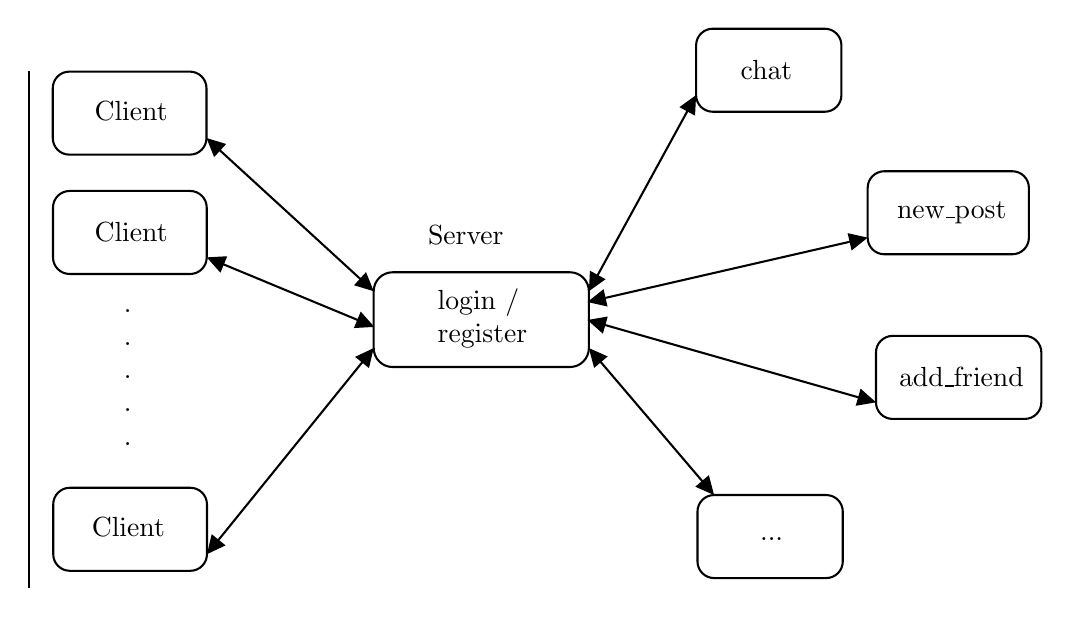
\begin{tikzpicture}[x=0.75pt,y=0.75pt,yscale=-1,xscale=1]
%uncomment if require: \path (0,300); %set diagram left start at 0, and has height of 300

%Rounded Rect [id:dp9287950498049711]
\draw   (90.7,40) .. controls (90.7,35.58) and (94.28,32) .. (98.7,32) -- (156.77,32) .. controls (161.19,32) and (164.77,35.58) .. (164.77,40) -- (164.77,64) .. controls (164.77,68.42) and (161.19,72) .. (156.77,72) -- (98.7,72) .. controls (94.28,72) and (90.7,68.42) .. (90.7,64) -- cycle ;
%Rounded Rect [id:dp49785700289931945]
\draw   (90.82,97.5) .. controls (90.82,93.08) and (94.4,89.5) .. (98.82,89.5) -- (156.88,89.5) .. controls (161.3,89.5) and (164.88,93.08) .. (164.88,97.5) -- (164.88,121.5) .. controls (164.88,125.92) and (161.3,129.5) .. (156.88,129.5) -- (98.82,129.5) .. controls (94.4,129.5) and (90.82,125.92) .. (90.82,121.5) -- cycle ;
%Rounded Rect [id:dp24820698998218682]
\draw   (90.93,240.5) .. controls (90.93,236.08) and (94.52,232.5) .. (98.93,232.5) -- (157,232.5) .. controls (161.42,232.5) and (165,236.08) .. (165,240.5) -- (165,264.5) .. controls (165,268.92) and (161.42,272.5) .. (157,272.5) -- (98.93,272.5) .. controls (94.52,272.5) and (90.93,268.92) .. (90.93,264.5) -- cycle ;
%Straight Lines [id:da6431591097520244]
\draw    (79.12,31.5) -- (79.12,280.75) ;
%Rounded Rect [id:dp012045389437388865]
\draw   (245.33,137.8) .. controls (245.33,132.76) and (249.42,128.67) .. (254.47,128.67) -- (339.87,128.67) .. controls (344.91,128.67) and (349,132.76) .. (349,137.8) -- (349,165.2) .. controls (349,170.24) and (344.91,174.33) .. (339.87,174.33) -- (254.47,174.33) .. controls (249.42,174.33) and (245.33,170.24) .. (245.33,165.2) -- cycle ;
%Straight Lines [id:da23180193797184767]
\draw    (166.98,66.03) -- (243.12,135.77) ;
\draw [shift={(245.33,137.8)}, rotate = 222.49] [fill={rgb, 255:red, 0; green, 0; blue, 0 }  ][line width=0.08]  [draw opacity=0] (8.93,-4.29) -- (0,0) -- (8.93,4.29) -- cycle    ;
\draw [shift={(164.77,64)}, rotate = 42.49] [fill={rgb, 255:red, 0; green, 0; blue, 0 }  ][line width=0.08]  [draw opacity=0] (8.93,-4.29) -- (0,0) -- (8.93,4.29) -- cycle    ;
%Straight Lines [id:da47978553629722653]
\draw    (167.65,122.65) -- (242.9,153.85) ;
\draw [shift={(245.67,155)}, rotate = 202.52] [fill={rgb, 255:red, 0; green, 0; blue, 0 }  ][line width=0.08]  [draw opacity=0] (8.93,-4.29) -- (0,0) -- (8.93,4.29) -- cycle    ;
\draw [shift={(164.88,121.5)}, rotate = 22.52] [fill={rgb, 255:red, 0; green, 0; blue, 0 }  ][line width=0.08]  [draw opacity=0] (8.93,-4.29) -- (0,0) -- (8.93,4.29) -- cycle    ;
%Straight Lines [id:da2079439502692908]
\draw    (166.89,262.17) -- (243.45,167.53) ;
\draw [shift={(245.33,165.2)}, rotate = 128.97] [fill={rgb, 255:red, 0; green, 0; blue, 0 }  ][line width=0.08]  [draw opacity=0] (8.93,-4.29) -- (0,0) -- (8.93,4.29) -- cycle    ;
\draw [shift={(165,264.5)}, rotate = 308.97] [fill={rgb, 255:red, 0; green, 0; blue, 0 }  ][line width=0.08]  [draw opacity=0] (8.93,-4.29) -- (0,0) -- (8.93,4.29) -- cycle    ;
%Rounded Rect [id:dp3595799346661108]
\draw   (400.67,19.33) .. controls (400.67,14.92) and (404.25,11.33) .. (408.67,11.33) -- (462.67,11.33) .. controls (467.08,11.33) and (470.67,14.92) .. (470.67,19.33) -- (470.67,43.33) .. controls (470.67,47.75) and (467.08,51.33) .. (462.67,51.33) -- (408.67,51.33) .. controls (404.25,51.33) and (400.67,47.75) .. (400.67,43.33) -- cycle ;
%Rounded Rect [id:dp8891537204147131]
\draw   (483.33,88) .. controls (483.33,83.58) and (486.92,80) .. (491.33,80) -- (553,80) .. controls (557.42,80) and (561,83.58) .. (561,88) -- (561,112) .. controls (561,116.42) and (557.42,120) .. (553,120) -- (491.33,120) .. controls (486.92,120) and (483.33,116.42) .. (483.33,112) -- cycle ;
%Rounded Rect [id:dp21536771570252933]
\draw   (487.33,167.33) .. controls (487.33,162.92) and (490.92,159.33) .. (495.33,159.33) -- (559,159.33) .. controls (563.42,159.33) and (567,162.92) .. (567,167.33) -- (567,191.33) .. controls (567,195.75) and (563.42,199.33) .. (559,199.33) -- (495.33,199.33) .. controls (490.92,199.33) and (487.33,195.75) .. (487.33,191.33) -- cycle ;
%Rounded Rect [id:dp4309981844331363]
\draw   (401.33,244) .. controls (401.33,239.58) and (404.92,236) .. (409.33,236) -- (463.33,236) .. controls (467.75,236) and (471.33,239.58) .. (471.33,244) -- (471.33,268) .. controls (471.33,272.42) and (467.75,276) .. (463.33,276) -- (409.33,276) .. controls (404.92,276) and (401.33,272.42) .. (401.33,268) -- cycle ;
%Straight Lines [id:da4183817050993175]
\draw    (350.95,167.48) -- (407.39,233.72) ;
\draw [shift={(409.33,236)}, rotate = 229.56] [fill={rgb, 255:red, 0; green, 0; blue, 0 }  ][line width=0.08]  [draw opacity=0] (8.93,-4.29) -- (0,0) -- (8.93,4.29) -- cycle    ;
\draw [shift={(349,165.2)}, rotate = 49.56] [fill={rgb, 255:red, 0; green, 0; blue, 0 }  ][line width=0.08]  [draw opacity=0] (8.93,-4.29) -- (0,0) -- (8.93,4.29) -- cycle    ;
%Straight Lines [id:da7230235815972146]
\draw    (351.22,152.49) -- (484.45,190.51) ;
\draw [shift={(487.33,191.33)}, rotate = 195.93] [fill={rgb, 255:red, 0; green, 0; blue, 0 }  ][line width=0.08]  [draw opacity=0] (8.93,-4.29) -- (0,0) -- (8.93,4.29) -- cycle    ;
\draw [shift={(348.33,151.67)}, rotate = 15.93] [fill={rgb, 255:red, 0; green, 0; blue, 0 }  ][line width=0.08]  [draw opacity=0] (8.93,-4.29) -- (0,0) -- (8.93,4.29) -- cycle    ;
%Straight Lines [id:da5565308194186631]
\draw    (351.26,142.33) -- (480.41,112.67) ;
\draw [shift={(483.33,112)}, rotate = 167.07] [fill={rgb, 255:red, 0; green, 0; blue, 0 }  ][line width=0.08]  [draw opacity=0] (8.93,-4.29) -- (0,0) -- (8.93,4.29) -- cycle    ;
\draw [shift={(348.33,143)}, rotate = 347.07] [fill={rgb, 255:red, 0; green, 0; blue, 0 }  ][line width=0.08]  [draw opacity=0] (8.93,-4.29) -- (0,0) -- (8.93,4.29) -- cycle    ;
%Straight Lines [id:da4459072101403143]
\draw    (350.44,135.17) -- (399.23,45.97) ;
\draw [shift={(400.67,43.33)}, rotate = 118.68] [fill={rgb, 255:red, 0; green, 0; blue, 0 }  ][line width=0.08]  [draw opacity=0] (8.93,-4.29) -- (0,0) -- (8.93,4.29) -- cycle    ;
\draw [shift={(349,137.8)}, rotate = 298.68] [fill={rgb, 255:red, 0; green, 0; blue, 0 }  ][line width=0.08]  [draw opacity=0] (8.93,-4.29) -- (0,0) -- (8.93,4.29) -- cycle    ;

% Text Node
\draw (123.5,145) node [anchor=north west][inner sep=0.75pt]   [align=left] {.\\.\\.\\.\\.};
% Text Node
\draw (270,104.67) node [anchor=north west][inner sep=0.75pt]   [align=left] {Server};
% Text Node
\draw (109.33,45) node [anchor=north west][inner sep=0.75pt]   [align=left] {Client};
% Text Node
\draw (109.33,103) node [anchor=north west][inner sep=0.75pt]   [align=left] {Client};
% Text Node
\draw (108,245) node [anchor=north west][inner sep=0.75pt]   [align=left] {Client};
% Text Node
\draw (274.67,135) node [anchor=north west][inner sep=0.75pt]   [align=left] {login /\\register};
% Text Node
\draw (420.67,25) node [anchor=north west][inner sep=0.75pt]   [align=left] {chat};
% Text Node
\draw (496,93) node [anchor=north west][inner sep=0.75pt]   [align=left] {new\textunderscore post};
% Text Node
\draw (497,173) node [anchor=north west][inner sep=0.75pt]   [align=left] {add\textunderscore friend};
% Text Node
\draw (430,255) node [anchor=north west][inner sep=0.75pt]   [align=left] {...};


\end{tikzpicture}

%-----------------------------------------------------
%sfarsit cod pentru diagrama
\newpage

\section{Aspecte de Implementare}
\subsection{Secțiuni de cod specifice}

\begin{mdframed}
    [linewidth=1pt, linecolor=black, topline=true, rightline=true, bottomline=true, leftline=true]
    \textbf{Comenzi implementate in server:}
    \begin{verbatim}
void CreateTable()
{
    char *sql = "CREATE TABLE IF NOT EXISTS users (id INTEGER PRIMARY KEY, email TEXT
    NOT NULL, password TEXT NOT NULL, username TEXT NOT NULL UNIQUE, friends TEXT,
    admin_key INTEGER, profile_type INTEGER, block INTEGER);";

    int rc = sqlite3_exec(db, sql, 0, 0, 0);
    if (rc != SQLITE_OK)
    {
        fprintf(stderr, "Cannot create table: %s\n", sqlite3_errmsg(db));
        exit(1);
    }

    sql = "CREATE TABLE IF NOT EXISTS posts (id INTEGER PRIMARY KEY, user_id INTEGER,
    content TEXT, post_type INTEGER, created_at DATETIME DEFAULT CURRENT_TIMESTAMP);";

    rc = sqlite3_exec(db, sql, 0, 0, 0);

    if (rc != SQLITE_OK)
    {
        fprintf(stderr, "Cannot create posts table: %s\n", sqlite3_errmsg(db));
        exit(1);
    }

    if (isAdminUserExisting() > 0) {
        printf("Admin user already exists.\n");
        return;
    }

    char password[] = "admin";
    Encrypt(password, encrypt_key);
    char insertAdminUserSQL[200];
    sprintf(insertAdminUserSQL, "INSERT INTO users (email, password, username, admin_key,
    profile_type) VALUES ('admin', '%s', 'admin', 1, 1);", password);

    rc = sqlite3_exec(db, insertAdminUserSQL, 0, 0, 0);

    if (rc != SQLITE_OK)
    {
        fprintf(stderr, "Cannot insert admin user: %s\n", sqlite3_errmsg(db));
        exit(1);
    }
}
    \end{verbatim}

\end{mdframed}

\begin{itemize}
    \item Serverul crează în baza de date SQLite3 tabelele: users - care v-a stoca toată informația despre utilizatorii înregistrați și tabela posts - care v-a stoca infromațiile despre postările tuturor utilizatorilor

    \item Serverul automat generează un utilizator admin cu privilegiile de administrator
\end{itemize}

\newpage

\begin{mdframed}
    [linewidth=1pt, linecolor=black, topline=true, rightline=true, bottomline=true, leftline=true]
    \textbf{Comenzi implementate in client:}
    \begin{verbatim}
    if (strcmp(buffer, "newpost") == 0)
    {
        printf("Enter your post: ");
        scanf(" %[^\n]", post);

        int post_size = strlen(post);
        send(client_sock, &post_size, sizeof(int), 0);

        send(client_sock, post, post_size, 0);

        Recv(client_sock, buffer, 1024, 0);
        printf("server: \t%s\n", buffer);
    }
    else if (strcmp(buffer, "login") == 0)
    {
        printf("Enter your username: ");
        scanf("%s", user_buffer);

        send(client_sock, user_buffer, strlen(user_buffer), 0);

        Recv(client_sock, buffer, 1024, 0);
        printf("server: \t%s\n", buffer);
    }
    \end{verbatim}

\end{mdframed}

\begin{itemize}

    \item Clientul introduce comenzi și le trimite la server prin "send".
    \item Se verifică tipul comenzii.
    \item Pentru comanda "login", clientul introduce numele de utilizator și îl trimite la server.
    \item pentru comanda "newpost", clientul introduce continutul postarii si il trimite la server.
    \item Răspunsul de la server cu privire la rezultatul functiei este afișat.

\end{itemize}

\subsection{Protocolul TCP}
Acest program are un server TCP concurent, ceea ce înseamnă că poate servi mai mulți clienți simultan, fiecare într-un proces sau într-un fir de execuție separat.
Iată câteva caracteristici ale serverului concurent:

\subsection*{Server Concurent}

\begin{itemize}

    \item \textbf{Multiprocessing sau Multithreading:} Un server concurent utilizează procese sau fire de execuție multiple pentru a manipula clienții simultan. Aceasta permite serverului să răspundă la cereri de la mai mulți clienți în același timp.

    \item \textbf{Performanță Îmbunătățită:} Serverul concurent are potențialul de a oferi performanțe mai bune decât serverul iterativ în situațiile în care există mai mulți clienți care trimit cereri în mod simultan. Astfel, se pot reduce timpii de așteptare pentru clienți.

    \item \textbf{Gestionarea Resurselor:} Serverul concurent poate gestiona eficient resursele, cum ar fi memoria și procesorul, prin împărțirea sarcinilor între mai multe procese sau fire de execuție. Acest lucru poate contribui la optimizarea utilizării resurselor sistemului.

\end{itemize}

\subsection{Scenarii reale de utilizare}

Programul este văzut ca un prototip al unei rețele de socializare, fiind capabilă să facă cele mai esențiale procese disponibile precum : crearea contului propriu, crearea postărilor, adăugarea prietenilor, comunicarea prin chat etc.

\section{Concluzii}

Proiectul VirtualSoc  propune o simulare  a unei rețele sociale, acoperind o gamă variată de funcționalități. Prin dezvoltarea acestuia, se pot dobândi cunoștințe valoroase în domeniul rețelelor sociale.

\subsection*{Potențiale îmbunătățiri ale proiectului}

\begin{itemize}

    \item adăugarea noilor funcționalități.
    \item optimizarea codului

\end{itemize}

\section{Bibliografie}

https://github.com/nikhilroxtomar/Multiple-Client-Server-Program-in-C-using-fork
\\
https://github.com/nikhilroxtomar/Chatroom-in-C
\\
https://www.sqlitetutorial.net

\end{document}
